\documentclass[border=1pt]{standalone}
% Shared preamble for the PixelRoot figures: Times text and math to match
% IEEEtran; every figure is drawn at its printed size (no scaling in the paper).
\usepackage[T1]{fontenc}
\usepackage{mathptmx}
\usepackage{amsmath}
\usepackage{xcolor}
\usepackage{tikz}
\usetikzlibrary{arrows.meta,positioning,calc,fit,backgrounds,decorations.pathreplacing,shapes.geometric}
\definecolor{ink}{HTML}{1B2838}
\definecolor{acc}{HTML}{1F5FBF}
\definecolor{grn}{HTML}{1E7B3A}
\definecolor{red}{HTML}{B3261E}
\definecolor{amb}{HTML}{9A6B00}
\definecolor{cu}{HTML}{B87333}
\tikzset{
  >={Stealth[length=1.6mm,width=1.2mm]},
  every picture/.style={line width=0.6pt, font=\footnotesize, color=ink},
  blk/.style={draw=ink, rounded corners=1.5pt, align=center, inner sep=2.5pt,
    minimum height=9mm, fill=white},
  note/.style={font=\scriptsize, align=left, text=ink!80},
}

\begin{document}
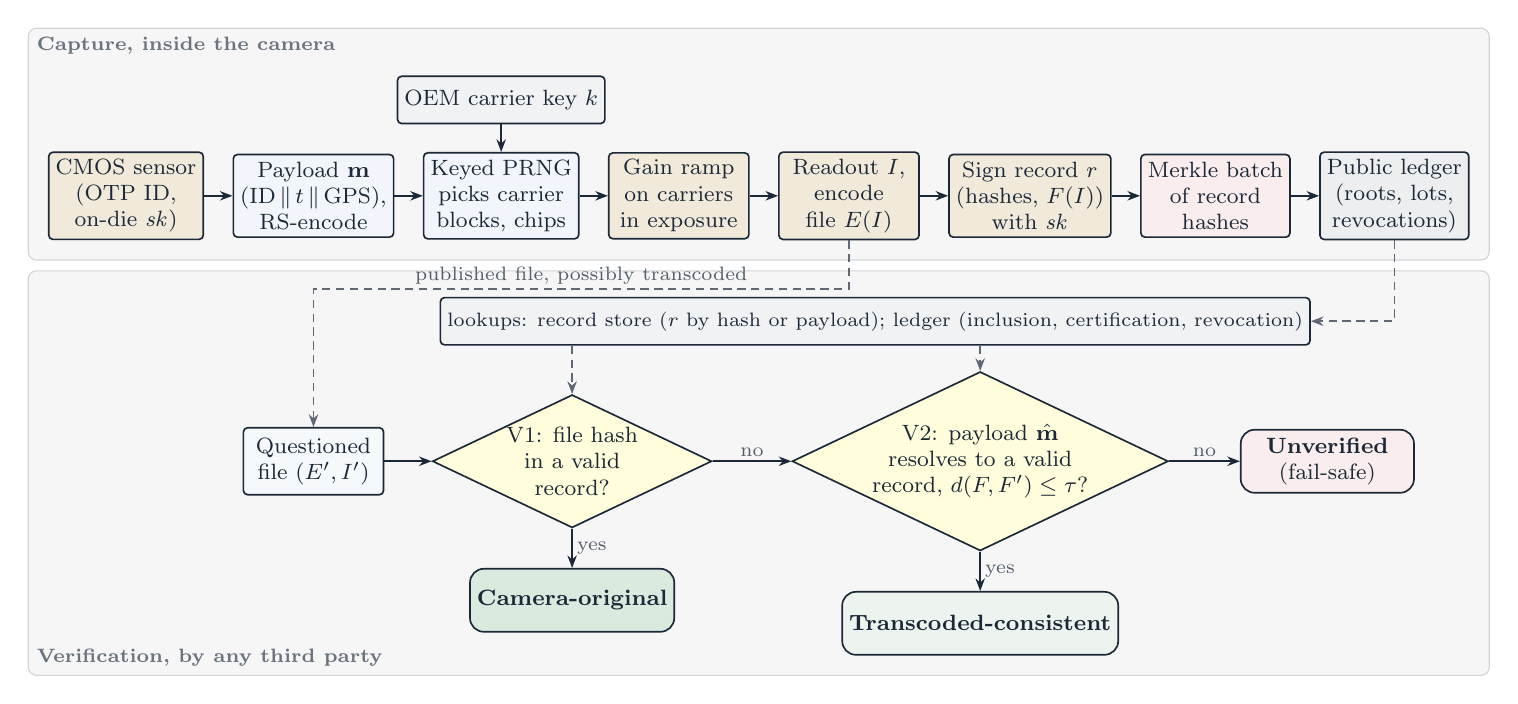
\begin{tikzpicture}[node distance=3.6mm]
\tikzset{
  s/.style={blk, minimum width=1.78cm, minimum height=1.05cm, fill=#1},
  s/.default=white,
  dec/.style={diamond, draw=ink, fill=yellow!14, aspect=2.1, inner sep=0.3pt, align=center},
  out/.style={blk, rounded corners=5pt, minimum width=2.2cm, minimum height=0.8cm, fill=#1},
  lane/.style={fill=ink!4, draw=ink!20, rounded corners=3pt},
  lanelab/.style={font=\scriptsize\bfseries, text=ink!65, anchor=north west, inner sep=3pt},
  dsh/.style={->, densely dashed, ink!70},
  lab/.style={font=\scriptsize, text=ink!75, inner sep=1.5pt},
}
% ---------------- capture lane
\node[s=amb!14] (sensor) {CMOS sensor\\(OTP ID,\\on-die $\mathit{sk}$)};
\node[s=acc!6, right=of sensor] (pay) {Payload $\mathbf m$\\(ID$\,\|\,t\,\|\,$GPS),\\RS-encode};
\node[s=acc!6, right=of pay] (prng) {Keyed PRNG\\picks carrier\\blocks, chips};
\node[s=amb!14, right=of prng] (gain) {Gain ramp\\on carriers\\in exposure};
\node[s=amb!14, right=of gain] (read) {Readout $I$,\\encode\\file $E(I)$};
\node[s=amb!14, right=of read] (sign) {Sign record $r$\\(hashes, $F(I)$)\\with $\mathit{sk}$};
\node[s=red!8, right=of sign] (merk) {Merkle batch\\of record\\hashes};
\node[s=ink!8, right=of merk] (led) {Public ledger\\(roots, lots,\\revocations)};
\node[s=ink!6, above=3.5mm of prng, minimum height=0.6cm] (key) {OEM carrier key $k$};
\foreach \a/\b in {sensor/pay, pay/prng, prng/gain, gain/read, read/sign, sign/merk, merk/led} \draw[->] (\a) -- (\b);
\draw[->] (key) -- (prng);
\coordinate (captop) at ($(key.north)+(0,0.35)$);
% ---------------- verification lane
\node[s=acc!4, below=24mm of pay, minimum height=0.85cm] (q) {Questioned\\file $(E', I')$};
\node[dec, right=6mm of q] (v1) {V1: file hash\\in a valid\\record?};
\node[dec, right=10mm of v1] (v2) {V2: payload $\hat{\mathbf m}$\\resolves to a valid\\record, $d(F,F')\le\tau$?};
\node[out=red!8, right=9mm of v2] (unv) {\textbf{Unverified}\\(fail-safe)};
\node[out=grn!16, below=5mm of v1] (orig) {\textbf{Camera-original}};
\node[out=grn!8, below=5mm of v2] (trans) {\textbf{Transcoded-consistent}};
\draw[->] (q) -- (v1);
\draw[->] (v1) -- node[above, lab] {no} (v2);
\draw[->] (v2) -- node[above, lab] {no} (unv);
\draw[->] (v1) -- node[right, lab] {yes} (orig);
\draw[->] (v2) -- node[right, lab] {yes} (trans);
% lookups used by both checks
\node[blk, fill=ink!6, minimum height=0.6cm, font=\scriptsize, anchor=south west]
  (look) at ($(v1.west |- v2.north)+(0.1,0.32)$) {lookups: record store ($r$ by hash or payload); ledger (inclusion, certification, revocation)};
\draw[dsh] (v1.north |- look.south) -- (v1.north);
\draw[dsh] (v2.north |- look.south) -- (v2.north);
\draw[dsh] (led.south) |- (look.east);
\draw[dsh] (read.south) -- ++(0,-0.62) -| node[pos=0.25, above, lab] {published file, possibly transcoded} (q.north);
% ---------------- lanes (background)
\coordinate (vertop) at ($(look.north)+(0,0.08)$);
\begin{scope}[on background layer]
  \node[lane, fit=(sensor)(led)(captop), inner sep=2.5mm] (cap) {};
  \node[lane, fit=(sensor.west |- vertop)(led.east |- trans.south), inner sep=2.5mm] (ver) {};
\end{scope}
\node[lanelab] at (cap.north west) {Capture, inside the camera};
\node[lanelab, anchor=south west] at (ver.south west) {Verification, by any third party};
\end{tikzpicture}
\end{document}
